\section{Componenti software}

Seguono le componenti software utilizzate e realizzate per raggiungere l'obiettivo.

\subsection{Kafka}

Apache Kafka è una piattaforma di streaming distribuita open-source
(Apache 2.0 \cite{apache2_license}) che svolge il ruolo di message broker
dove dei "producer" possono pubblicare messaggi, che verranno poi consumati per essere analizzati,
su specifici topic. Ciò consente a più producer di pubblicare su topic distinti o sul medesimo,
utile per esempio nel caso si desideri collezionare gli stessi dati da più fonti
(in questo contesto aggiungere fonti secondarie potrebbe frazionare il rischio relativo
all'interruzione dei dati riguardanti l'andamento della criptovaluta sul mercato).
\\
La scelta è ricaduta sul suddetto software perchè in grado di garantire
high-availability, fault-tolerancy, ottime performance e la possibilità di configurare un cluster
di più nodi scalabile quindi orizzontalmente. \cite{kafka_doc}
\\
In più grazie risulta ben integrato con Apache Spark, framework su cui si basa l'applicazione
analitica, semplificando la ricezione dei messaggi dal broker.

% La versione utilizzata è ...

\subsubsection{Zookeeper}

Apache Zookeeper è un software open-source, anch'esso distribuito sotto licenza
Apache 2.0 \cite{apache2_license}, che nasce come "coordinatore" di sistemi distribuiti
in grado di svolgere compiti come rendere disponibili configurazioni centralizzati ai vari
componenti distribuiti. Zookeeper è al momento richiesto da Kafka per memorizzare metadati
necessari al funzionamento del cluster \cite{kafka_zookeeper}.

\subsection{Producers}

Il ruolo dei producer consiste nel ricevere dati in streaming da determinate fonti e di
pubblicarli prontamente su di un topic Kafka.
\\
Entrambi i producer sono stati realizzati in python per semplicità nell'utilizzo delle
librerie fornite dalle fonti per l'acquisizione di dati in tempo reale.
\\
Allo scopo di valutare le performance dell'intero progetto entrambi i producer aggiungono
ad ogni messaggio un campo contenente l'esatto momento di ricezione.

\subsubsection{Binance producer}

Binance producer riceve dati dalla piattaforma di exchange Binance \cite{binance}
avvalendosi della libreria ufficiale per poi pubblicarli su Kafka.

\subsubsection{Tweets producer}

Tweets producer fa uso della libreria Tweepy \cite{tweepy} per ottenere tweets relativi
ad un determinato filtro e poi pubblicarli su Kafka.
\\
La logica di entrambi i producer si può riassumere nelle seguenti fasi:
\begin{enumerate}
    \item Connessione alla fonte di dati
    \item Connessione a Kafka
    \item Definizione di una funziona da effettuare al ricevimento di nuovi messaggi che
          principalmente si occuperà della pubblicazione del messaggio su Kafka
\end{enumerate}

Segue un estratto di codice da "Tweets producer":

\begin{lstlisting}[language=python,firstnumber=1]
# Connessione a Kafka
producer = kafka.KafkaProducer(
                bootstrap_servers=kafka_servers,
                value_serializer=lambda x: 
                json.dumps(x).encode('utf-8'))

class TweetsStreamListener(tweepy.StreamListener):
    # Definizione della funzione
    def on_status(self, tweet):
        if verbose:
            print(json.dumps(tweet._json))
        msg = tweet._json
        msg["receivedat"] = time.time()
        producer.send(kafka_topic, value=msg)

tweetsStreamListener = TweetsStreamListener()
# Connessione a Twitter
twStream = tweepy.Stream(auth = auth,
                listener=tweetsStreamListener)
twStream.filter(track=tweets_filter)
\end{lstlisting}

\subsection{TimescaleDB}

TimescaleDB è un database relazionale open-source ottimizzato per dati di tipo time-series
offrendo strutture adeguate al tipo di dati così da incrementare le performance dalla ricerca
all'inserimento fino allo storage; ad esempio permette di impostare un intervallo di tempo
dopo il quale i dati vengono compressi \cite{timescale}.
\\
Si basa su PostgreSQL, noto database relazionale open-source \cite{postgresql}, più precisamente
ne è un estensione. Per questo motivo TimescaleDB risulta relativamente semplice da utilizzare
per coloro che hanno già avuto esperienza con PostgreSQL ed è inoltre compatibile con i client
supportati da PostgreSQL.
\\
Ciò semplifica la connessione con l'applicazione Spark che grazie al module Spark SQL è in grado
di utilizzare driver JDBC per intergire con database relazionali tra cui PostgreSQL
\cite{spark_sql}.

\subsection{Spark}

Apache Spark è un framework open-source per l'analisi di dati su larga scala che offre ottime
performance sia per elaborazioni batch che in streaming. Offre API di alto livello nei lingiaggi
Scala, Java, Python e R, e librerie aggiuntive come MLlib, che fornisce strumenti utili per il
machine learning, Spark SQL, modulo per l'elaborazione di dati strutturati,
e Structured Streaming basato su Spark SQL ma rivolto ai dati strutturati in streaming \cite{spark}.
\\
Le API Spark consentono di sviluppare applicazioni scalabili orizzontalmente, highly-available
e fault-tolerant; infatti possono
essere eseguite su cluster comprendenti diverse macchine tra cui almeno un \textbf{master} ed un
\textbf{worker}.
\\
Spark risulta decisamente più performante del paradigma MapReduce soprattutto per quegli algoritmi
che necessitano ripetute letture degli stessi dati per il fatto che al contrario di MapReduce non
necessita di rileggere i dati da disco ma utilizza una cache in memoria \cite{spark_mapred}.

\subsubsection{StreamApp}

Applicazione sviluppata utilizzando le API Scala di Apache Spark. Rappresenta il cuore del progetto:
si occupa di ricevere, elaborare e analizzare sia i dati finanziari che i tweets.

\subsubsection{TrainApp}

Applicazione aggiuntiva anch'essa sviluppata utilizzando le API Scala di Apache Spark che si occupa
del training di alcuni modelli utilizzati da StreamApp a partire dai dati ricevuti da essa.
Per questo motivo StreamApp è necessariamente in grado di funzionare (parzialmente) anche in assenza
di questi modelli cossicchè sia possibile ottenere una quantità di dati iniziale con cui allenare i
modelli.

\subsection{Grafana}

Grafana è un software open-source che si occupa di operazioni di visualizzazione e analitiche
di dati tra cui serie temporali. È qui utilizzato come dashboard per eseguire query verso
TimescaleDB e permetterne una semplice e completa visualizzazione dei risultati.

\begin{figure}[h!]
    \centering
    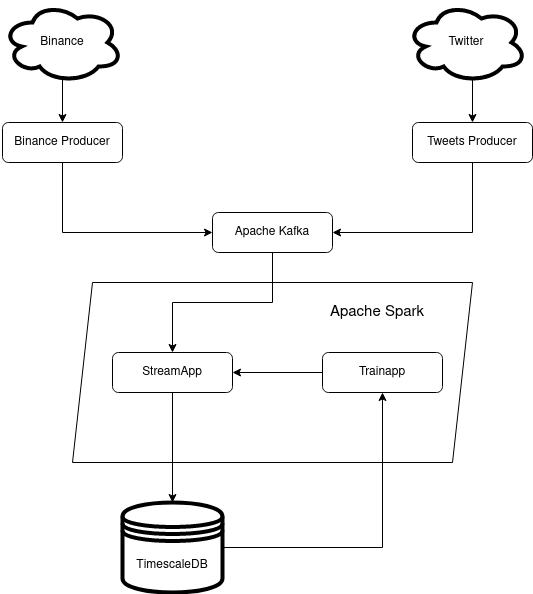
\includegraphics[
		height=10cm,
		keepaspectratio,
    ]{ad_schema.png}
    \caption{Schema delle componenti principali}
\end{figure}

% schema grafico
% docker-compose
